\subsection{Protocolos de intera\c{c}\~oes}
\label{section:protocolos_interacoes}
\begin{figure}[h]
\caption{Tipos de relacionamentos}
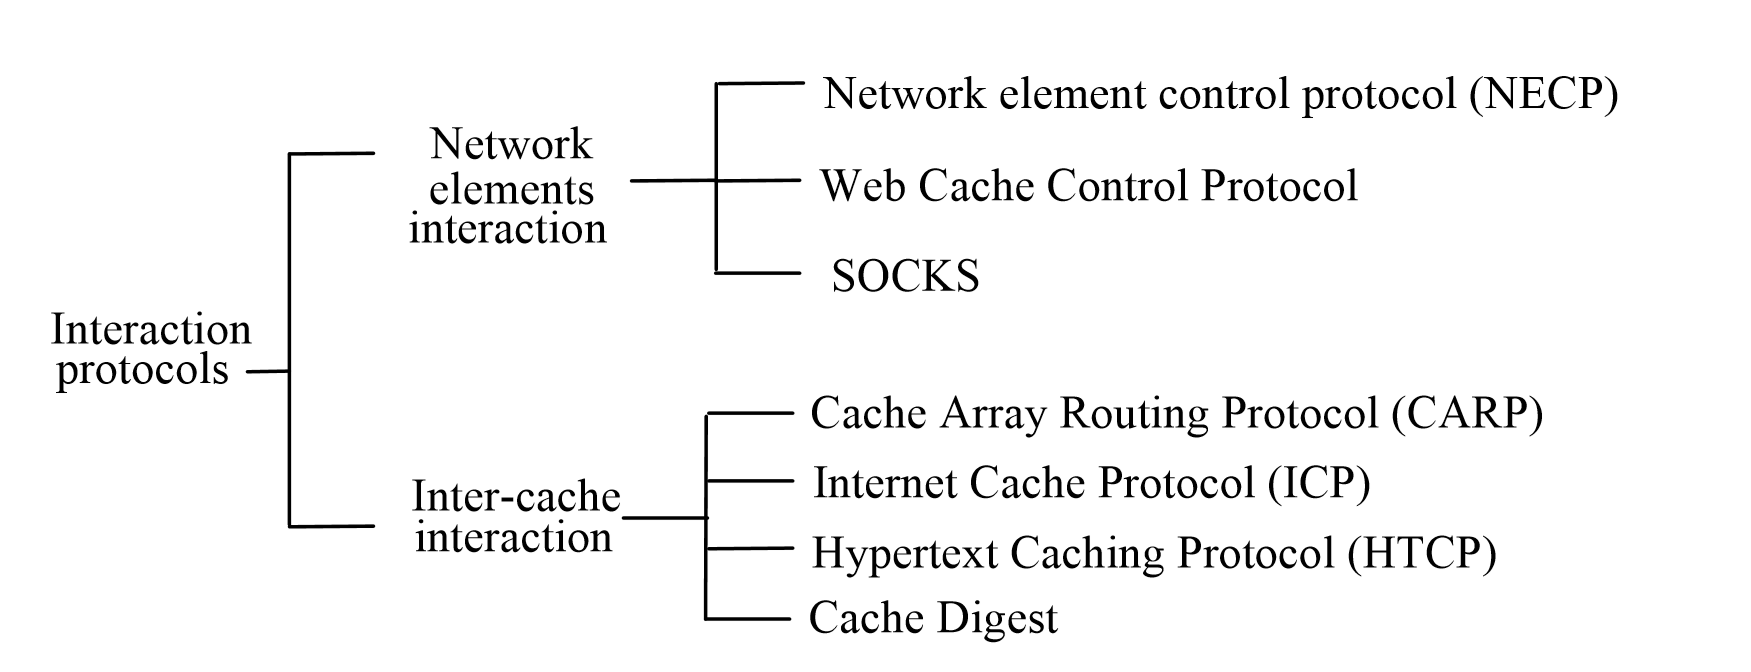
\includegraphics[width=10cm]{Figuras/tipos_relacionamentos.png} 
\label{figura:tipos_relacionamentos}
\end{figure}

\paragraph{} Os protocolos de intera\c{c}\~oes podem ser divididos em duas partes: Protocolos de intera\c{c}\~oes de elementos da rede e Protocolos de intera\c{c}\~oes entre os servidores de cache da CDN. 


\subsubsection{Intera\c{c}\~oes dos elementos da rede}
\begin{figure}[h]
\caption{Tipos de protocolos de itera\c{c}\~oes}
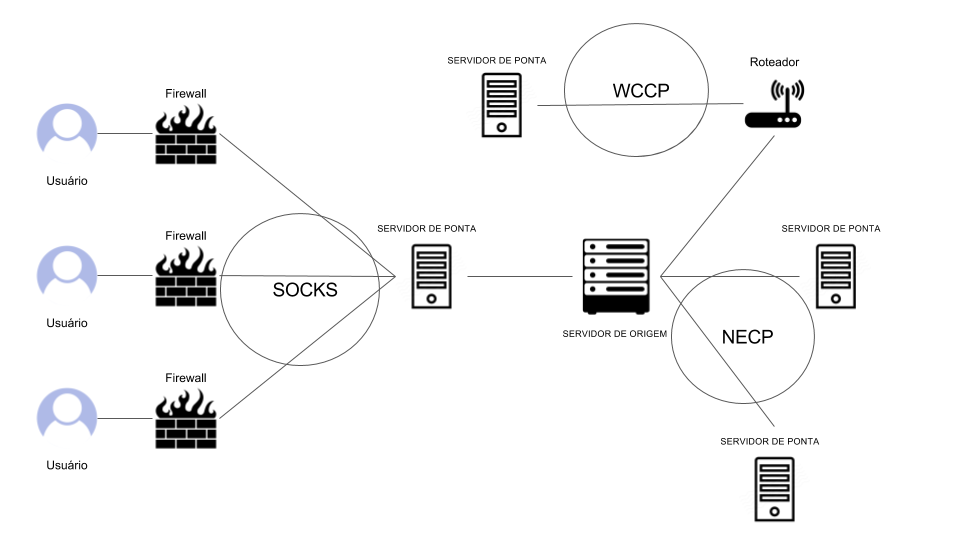
\includegraphics[width=10cm]{Figuras/protocolos_interacao_elementos.png} 
\label{figura:protocolos_interacao_elementos}
\end{figure}

\paragraph{} Dentro dos protocolos de intera\c{c}\~oes dos elementos de rede podemos verificar que cada um possui sua especificidade e funcionalidade bem definida, como podemos ver na figura \ref{figura:protocolos_interacao_elementos} , tentando proteger o n\~ao s\'o a rede mas tamb\'em o usu\'ario, o servidor, os roteadores e a comunica\c{c}\~ao entre os mesmos.


\subsubsection{Intera\c{c}\~oes de cache}

\paragraph{} Os protocolos de intera\c{c}\~oes de cache s\~ao protocolos que organizam as trocas de informa\c{c}\~oes entre os servidores, ou seja, \'e ele que dita como ir\'a funcionar a distribui\c{c}\~ao da informa\c{c}\~ao dentro da rede.
\paragraph{} Conforme vimos na figura \ref{figura:tipos_relacionamentos}, e segundo \cite{pathan2007taxonomy}, existem 4 tipos de protocolos aplicados nessa circunst\^ancia, que s\~ao:
\begin{itemize}
\item HTCP - Hypertext Caching Protocol
\item ICP - Internet Cache Protocol
\end{itemize}
\paragraph{} Ambos s\~ao concorrentes entre s\'i e tem como funcionalidade controlar o fluxo de informa\c{c}\~ao entre os caches. Sendo atrav\'es deles que se controla o que ir\'a para um determinado servidor de ponta, por exemplo. Falaremos mais sobre ambos em \ref{section:HTCP} e \ref{section:ICP} respectivamente.
\paragraph{} Existe tamb\'em os protocolos:
\begin{itemize}
\item CARP -  Cache Array Routing Protocol
\item Cache Digest
\end{itemize}
\paragraph{} Esses dois protocolos, tamb\'em concorrentes entre s\'i, servem para controlar o conte\'udo existente dentro de cada servidor e saber onde est\~ao os outros conte\'udos. Falaremos mais sobre ambos em \ref{section:CARP} e \ref{section:Cache Digest} respectivamente.

\subsubsection{HTCP}
\label{section:HTCP}
\paragraph{} Como dito anteriormente o HTCP, Hypertext Caching Protocol, \'e um protocolo de intera\c{c}\~ao entre os caches, suas principais caracterist\'icas s\~ao:
\begin{itemize}
\item Protocolo para descobri Caches HTTP;
\item Suporte ao HTTP 1.0;
\item Permite incluir cabeçalhos nas respostas;
\item Podem ser enviados via TCP/UDP;
\item Devem ser resilientes \`a falhas.
\end{itemize}

\subsubsection{ICP}
\label{section:ICP}
\paragraph{} J\'a o ICP, Internet Cache Protocol, \'e um protocolo muito mais leve que possui as seguintes caracterist\'icas:
\begin{itemize}
\item Protocolo de mensagem leve;
\item Utilizado para comunica\c{c}\~ao de Caches;
\item Utiliza consultas para determinar localiza\c{c}\~ao mais apropriada;
\item Suporte ao HTTP 0.9;
\item Comunica-se com caches vizinhos;
\item recebe MISS ou HIT como resposta;
\item Enviado via UDP;
\item Falha por timeout indica caminho quebrado;
\item Fornece informa\c{c}\~oes para balanceamento atrav\'es das medidas de perda.
\end{itemize}

\subsubsection{HTCP x ICP}
\paragraph{} Analisando os dois protocolos,HTCP e ICP, podemos fazer um quadro comparativo entre os e coloc\'a-los da seguinte maneira(figura \ref{figura:htcp_x_icp}):

\begin{figure}[h]
\caption{HTCP x ICP}
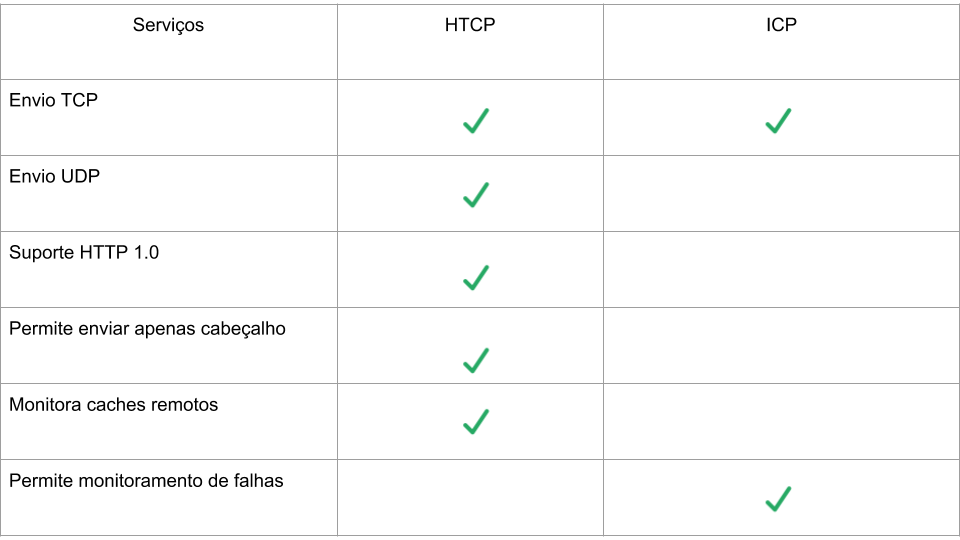
\includegraphics[width=10cm]{Figuras/htcp_x_icp.png} 
\label{figura:htcp_x_icp}
\end{figure}

\subsubsection{CARP}
\label{section:CARP}
CARP -  Cache Array Routing Protocol
\paragraph{} Protocolo de armazenamento distribu\'ido baseado em uma lista conhecida de proxies suavemente acoplada e uma fun\c{c}\~ao hash para dividir o espa\c{c}o URL entre esses proxies.
\begin{itemize}
\item Cliente HTTP pode enviar requisi\c{c}\~ao \`a qualquer proxy da lista.
\end{itemize}

\subsubsection{Cache Digest}
\label{section:Cache Digest}
Cache Digest
\paragraph{} Protocolo de interc\^ambio e formato de dados entre caches.
\begin{itemize}
\item Fornecem um resumo dos conte\'udos na resposta;
\item Soluciona os problemas de congestionamento e timeout;
\item Torna poss\'ivel determinar se um servidor possui em cache um conte\'udo;
\item Executado via HTTP ou FTP;
\item Cont\'em tempo de expira\c{c}\~ao na resposta;
\item Podem ser utilizados para eliminar redund\^ancia.
\end{itemize}
